%%%%%%%%%%%%%%%%%%%%%%%%%%%%%%%%%%%%%%%%%%%%%%%%%%%%%%%%%%%%%%%%%%%%%
%% PhaseFoundry JOSS paper
%% PhaseFoundry paper, Attari & Arróyave, 2025
%%%%%%%%%%%%%%%%%%%%%%%%%%%%%%%%%%%%%%%%%%%%%%%%%%%%%%%%%%%%%%%%%%%%%
\documentclass[12pt]{article}

\usepackage[T1]{fontenc}
\usepackage[utf8]{inputenc}
\usepackage{microtype}
\usepackage{helvet}           % RSC uses sans-serif headings
\usepackage{times}            % Times body text
\usepackage[margin=2cm,top=2.5cm,bottom=2.5cm]{geometry}
\usepackage{amsmath,amssymb}
\usepackage{graphicx}
\usepackage{booktabs}
\usepackage{xcolor}
\usepackage{hyperref}
\usepackage[numbers,super,sort&compress]{natbib}
\usepackage{caption}
\usepackage{listings}
\usepackage{enumitem}
\usepackage{fancyhdr}
\setlength{\headheight}{13.6pt}
\addtolength{\topmargin}{-1.6pt}
\usepackage{abstract}
\usepackage{titlesec}
\usepackage{siunitx}
\usepackage{rotating}
\usepackage{float}
\usepackage[percent]{overpic}

%% ── RSC-style heading formatting ─────────────────────────────────
\titleformat{\section}{\sffamily\bfseries\large}{\thesection}{0.5em}{}
\titleformat{\subsection}{\sffamily\bfseries\normalsize}{\thesubsection}{0.5em}{}
\titleformat{\subsubsection}{\sffamily\itshape\normalsize}{\thesubsubsection}{0.5em}{}
\titlespacing*{\section}{0pt}{10pt}{4pt}
\titlespacing*{\subsection}{0pt}{8pt}{3pt}

%% ── Caption style ────────────────────────────────────────────────
\captionsetup{font=small, labelfont=bf, labelsep=period}

%% ── Code listings ────────────────────────────────────────────────
\lstdefinelanguage{yaml}{
  keywords={true,false,null},
  keywordstyle=\color{blue!70}\bfseries,
  comment=[l]{\#},
  commentstyle=\color{gray}\itshape,
  morestring=[b]',
  morestring=[b]",
  stringstyle=\color{orange!80!black},
  sensitive=false,
}

\lstset{
  basicstyle=\ttfamily\fontsize{6.3}{7.6}\selectfont,
  backgroundcolor=\color{gray!8},
  frame=single,
  framerule=0.4pt,
  breaklines=true,
  columns=flexible,
  xleftmargin=0.1\columnwidth,
  xrightmargin=0.1\columnwidth,
}

%% ── Header / footer ──────────────────────────────────────────────
\pagestyle{fancy}
\fancyhf{}
\fancyhead[LE,RO]{\small\thepage}
\fancyhead[RE]{\small\itshape PhaseFoundry}
\fancyhead[LO]{\small\itshape Attari \& Arr\'oyave}
\renewcommand{\headrulewidth}{0.4pt}

%% ─────────────────────────────────────────────────────────────────
\begin{document}

%% ── Title block ──────────────────────────────────────────────────

\vspace*{4pt}
{\noindent\LARGE\sffamily\bfseries
PhaseFoundry: An Open-Source CALPHAD-Coupled Phase-Field Framework\\
for Spinodal Microstructure Design in Multicomponent Alloys}

\vspace{12pt}

{\noindent\large
Vahid Attari$^{a}$ and Raymundo Arr\'oyave$^{a,b,c}$}

\vspace{6pt}

{\noindent\small
$^{a}$Department of Materials Science and Engineering, Texas A\&M University,
College Station, TX~77843, USA\\
$^{b}$J.\ Mike Walker~'66 Department of Mechanical Engineering, Texas A\&M University,
College Station, TX~77843, USA\\
$^{c}$Wm Michael Barnes~'64 Department of Industrial and Systems Engineering,
Texas A\&M University, College Station, TX~77843, USA\\[3pt]
Correspondence: \href{mailto:attari.v@tamu.edu}{attari.v@tamu.edu}}

\vspace{10pt}

%% ── Abstract ─────────────────────────────────────────────────────
\noindent\rule{\linewidth}{1pt}
\vspace{4pt}

\noindent\textbf{Abstract.}\quad
Predicting how a multicomponent alloy decomposes into a nanoscale two-phase microstructure requires connecting thermodynamic databases, which encode where a solid solution is unstable, to phase-field simulations, which resolve how that instability evolves in space and time. In practice this connection is the weakest link in the integrated computational materials engineering (ICME) toolchain: free energy models are hand-transcribed into solver source code, chemical potentials are approximated by finite differences, and coherency strain effects are either neglected or parameterized \textit{ad hoc}. We present \textit{PhaseFoundry}, an open-source Python framework that closes this gap for spinodal microstructure design. Starting from a CALPHAD thermodynamic database -- including databases generated from machine-learned interatomic potentials (MLIPs) via \textit{PhaseForge} -- the framework evaluates exact Gibbs energy Hessians and chemical potentials using analytic Jansson derivatives in \textit{pycalphad}, maps spinodal instability regions through gauge-invariant eigenanalysis, and evolves the resulting instabilities with an unconditionally stable pseudo-spectral Cahn--Hilliard solver that optionally includes coherency strain via a Moulinec--Suquet spectral micromechanics solver with MLIP-derived, composition-dependent elastic constants. Binary, ternary, and quaternary alloy systems are specified entirely through YAML configuration files, with no code changes. \textit{PhaseFoundry} is available under the MIT license at \url{https://github.com/vahid2364/PhaseFoundry}.

\vspace{4pt}
\noindent\rule{\linewidth}{1pt}
\vspace{10pt}


%% ── 1. Introduction ──────────────────────────────────────────────
\section{Introduction}

Spinodal decomposition, the barrierless unmixing of a supersaturated solid solution into compositionally modulated domains by uphill diffusion, has been understood thermodynamically since Gibbs\cite{gibbs1878equilibrium} and given its modern continuum formulation by Cahn and Hilliard.\cite{cahn1958free,cahn1961spinodal} It has recently reemerged as a deliberate microstructure design strategy. Depending on the alloy, the transformation can be harmful, embrittling otherwise ductile solid solutions\cite{wang2023spinodal} or providing a pathway for deleterious ordered phases,\cite{dasari2023crystallographic} or it can be exploited: in refractory and 3d-transition-metal high-entropy alloys (HEAs), spinodally modulated solid solutions have been shown to overcome the strength-ductility trade-off,\cite{an2021spinodal,zhang2022refinement,lee2025spinodal} tailor magnetic properties,\cite{rao2021beyond,dong2024cooperative} and improve thermoelectric performance.\cite{duan2025spinodal} Either way, the designer must first locate the spinodal region within a vast, high-dimensional composition space, and then predict the morphology, length scale, and phase compositions of the resulting microstructure.

The thermodynamic half of the problem is well served by mature tools. CALPHAD databases encode assessed Gibbs energy models for multicomponent phases, and both commercial engines such as Pandat\cite{cao2009pandat} and open-source engines such as \textit{pycalphad}\cite{otis2017pycalphad} make these models programmatically accessible, with ESPEI providing automated database development and uncertainty quantification.\cite{bocklund2019espei} Where classical assessments do not exist, \textit{PhaseForge}\cite{sariturk2025phaseforge,zhu2025accelerating,zhu2025machine} has recently emerged as a dedicated open-source toolkit that automates the construction of CALPHAD-compatible TDB files for arbitrary multicomponent alloy systems using machine-learned interatomic potentials (MLIPs). Starting from a set of DFT-informed MLIP calculations, \textit{PhaseForge} generates thermodynamic interaction parameters, SQS-based elastic constant tables, and lattice parameter data -- all in formats directly consumable by downstream simulation tools such as \textit{PhaseFoundry} -- at a fraction of the cost of conventional density functional theory assessments.\cite{kunselman2025construction} This MLIP-to-TDB pipeline substantially lowers the barrier to constructing thermodynamic databases for novel HEA systems that lack experimental assessments. The stability analysis needed to locate spinodal regions has a long lineage, from de Fontaine's coherent stability criteria\cite{de1967computer,de1972analysis} through Gibbs energy Hessian analysis for HEAs\cite{morral2021stability} and high-throughput CALPHAD-based spinodal screening.\cite{koneru2022high,kadirvel2022exploration} The kinetic half is likewise well served by general-purpose phase-field frameworks such as MOOSE,\cite{permann2020moose} PRISMS-PF,\cite{dewitt2020prisms} and FiPy.\cite{guyer2009fipy}

The difficulty lies in two distinct coupling problems. The first is thermodynamic: a running phase-field simulation queries the free energy and its composition derivatives at every grid point and every time step, yet general-purpose frameworks require users to supply these functions explicitly. Direct CALPHAD equilibrium calls are feasible for binary systems but become prohibitively expensive as the number of components grows, since each call invokes a Gibbs minimization whose cost scales steeply with the number of species and solution phases. For multicomponent CALPHAD phases this means either hand-fitting polynomial surrogates that drift from the database, or numerically differentiating equilibrium calculations with finite differences -- an approach sensitive to stencil size and increasingly unreliable in high-dimensional composition spaces.\cite{kunselman2024analytically} The second is elastic: coherency strain, which shrinks the effective spinodal region\cite{cahn1961spinodal,de1972analysis} and governs decomposition morphology, requires composition-dependent elastic constants and eigenstrain coefficients that are not tabulated for most multicomponent alloy systems and are not a natural output of any CALPHAD database.

In this work, we present \textit{PhaseFoundry}, an open-source Python framework built on our recently developed CALPHAD-coupled phase-field methodology.\cite{attari2021strain,attari2023uncertainty,attari2020exploration,attari2023benchmarking,kunselman2025spinodal} \textit{PhaseFoundry} circumvents the free energy coupling bottleneck by introducing a pre-computed scattered-data surrogate, constructed once from thermodynamic derivatives evaluated on a composition grid, that serves as the sole thermodynamic object queried at runtime. Three derivative modes are available and selectable via the configuration file: analytic Jansson derivatives\cite{kunselman2024analytically} (the default, exact to machine precision), finite differences on pycalphad equilibrium calls (for validation and backward compatibility), and a hybrid mode that combines both for cross-checking. This surrogate enables the incorporation of exact CALPHAD thermodynamics within the phase-field framework for multicomponent solid solutions spanning binary to quaternary systems, without hand-transcribed free energy functions or finite-difference approximations.

One major advantage of \textit{PhaseFoundry} is the simultaneous treatment of thermodynamic driving forces and coherency strain within a single, configuration-driven pipeline. This advantage arises from the combined use of gauge-invariant Hessian eigenanalysis\cite{kadirvel2022exploration,morral2021stability} and SQS/MLIP-derived composition-dependent elastic constants,\cite{zunger1990special} which together enable an accurate representation of both the chemical instability and the elastic energy landscape across the full composition space of a multicomponent alloy. \textit{PhaseFoundry} therefore provides a more practical approach to spinodal microstructure prediction compared to workflows that treat thermodynamics and elasticity as separate, manually parameterized inputs,\cite{permann2020moose,dewitt2020prisms} and eliminates the need for DFT recalculation of elastic properties at each new composition of interest by interpolating from a pre-computed MLIP table.

A number of capable software tools have been developed to address parts of this problem. MOOSE\cite{permann2020moose} and PRISMS-PF\cite{dewitt2020prisms} provide mature, massively parallel finite-element phase-field infrastructure with broad multiphysics scope; CALPHAD coupling in these frameworks typically relies on user-supplied polynomial free energy expressions rather than direct TDB evaluation. FiPy\cite{guyer2009fipy} offers a flexible, accessible PDE specification layer well suited to rapid prototyping. OpenPhase and the commercial code MICRESS, coupled to Thermo-Calc, support sophisticated multi-phase, multi-component simulations and are widely used in the solidification and grain-growth communities. These tools collectively cover a wide range of microstructure problems; none, however, provides automated, composition-dependent elastic parameterization from first-principles or MLIP data: elastic constants and eigenstrain coefficients must be supplied externally by the user.

\textit{PhaseFoundry} can be distinguished from the aforementioned tools in two respects. First, it couples a CALPHAD thermodynamic database directly to the phase-field solver through analytic Jansson derivatives\cite{kunselman2024analytically} and a pre-computed free-energy surrogate, eliminating both finite-difference error and the cost of repeated Gibbs minimizations at runtime; binary, ternary, and quaternary systems are handled by the same code path with no user-supplied free energy functions. Second, it integrates composition-dependent elastic constants derived from SQS/MLIP calculations\cite{zunger1990special} into a Moulinec--Suquet spectral elasticity solver,\cite{moulinec1998numerical} so that coherency strain enters the simulation with the same level of automation as the thermodynamics. Together these two features complete an open-source, reproducible pipeline from a CALPHAD TDB to a quantitative elasto-chemical spinodal microstructure, driven entirely by a single YAML configuration file. This is particularly consequential for high-throughput HEA design, where spinodal decomposition is both a target phenomenon and a screening criterion: the ability to rapidly sweep composition space, identify spinodal windows, and predict the resulting microstructure morphology and length scale -- all from a single thermodynamic database and without per-alloy manual parameterization -- transforms what has been a laborious case-by-case simulation task into a scalable design loop. A companion paper\cite{kunselman2025spinodal} presents the scientific application of this pipeline to the Hf--Nb--Ti--V refractory HEA system.

In the following sections, we provide a brief description of the theoretical framework underlying \textit{PhaseFoundry}, a concise overview of the software architecture and configuration system, a detailed description of the numerical implementation, and illustrative applications across binary, ternary, and quaternary alloy systems. The source code, documentation, and all configuration files used in this work are openly available at \url{https://github.com/vahid2364/PhaseFoundry}.

%% ── 2. Theoretical framework ─────────────────────────────────────
\section{Theoretical framework}

\subsection{Spinodal stability and the Gibbs energy Hessian}

For an $n$-component solid solution phase $\alpha$, the condition for spinodal instability is that at least one eigenvalue of the molar Gibbs energy Hessian,
\begin{equation}
  H_{ij} = \frac{\partial^2 G_m^\alpha}{\partial x_i \,\partial x_j}, \quad i,j = 1,\ldots,n-1,
\end{equation}
is negative.\cite{cahn1961spinodal,de1972analysis} When coherency strain is present, the relevant quantity is the coherent Hessian,\cite{cahn1961spinodal}
\begin{equation}
  H_{ij}^{\rm coh} = H_{ij} + \eta_{ij}^{\rm el},
\end{equation}
where $\eta_{ij}^{\rm el}$ is the elastic stiffening contribution from coherency misfit, which always stabilizes the solid solution relative to the purely chemical criterion. The spinodal boundary in composition space is the locus where the smallest eigenvalue of $H^{\rm coh}$ passes through zero.

Because $H_{ij}$ depends on the choice of dependent component, \textit{PhaseFoundry} transforms it to a gauge-invariant Cartesian basis before eigenanalysis,\cite{kadirvel2022exploration,morral2021stability} ensuring that spinodal boundaries and instability directions are independent of the labeling convention. For systems with four or more components, the resulting instability maps are visualized using affine projections of the composition simplex.\cite{vela2025visualizing}

\subsection{CALPHAD free energy and analytic derivatives}

The molar Gibbs energy $G_m^\alpha(\mathbf{x}, T)$ is provided by a CALPHAD thermodynamic database, which encodes the Gibbs energy of each phase as a function of composition and temperature through assessed interaction parameters.\cite{lukas2007computational} Evaluating $H_{ij}$ by numerical differentiation of equilibrium CALPHAD calculations is both costly and sensitive to the finite-difference stencil in high-dimensional composition spaces.\cite{kunselman2024analytically} \textit{PhaseFoundry} instead uses the Jansson derivative method,\cite{kunselman2024analytically} which propagates analytic derivatives of the Gibbs energy through the equilibrium conditions to yield exact chemical potentials and Hessian elements at negligible additional cost relative to a single equilibrium call. The derivatives are evaluated on a composition grid and stored; a scattered-data surrogate (RBF or polynomial, fit once) serves as the sole thermodynamic object queried during the phase-field simulation.

\subsection{Cahn--Hilliard phase-field model}

The temporal evolution of the $n-1$ independent mole-fraction fields $x_i(\mathbf{r},t)$ follows the multicomponent Cahn--Hilliard equations,\cite{cahn1958free}
\begin{equation}
  \frac{\partial x_i}{\partial t} = \nabla \cdot \sum_{j=1}^{n-1} M_{ij}(\mathbf{x})\,\nabla \mu_j^{\rm tot},
\end{equation}
derived from the free energy functional
\begin{equation}
  \mathcal{F}[\mathbf{x}] = \int_\Omega \!\left[ G_m^\alpha(\mathbf{x}) + \sum_{i=1}^{n-1} \frac{\kappa_i}{2}|\nabla x_i|^2 \right] dV.
\end{equation}
The total chemical potential $\mu_j^{\rm tot} = \partial G_m^\alpha/\partial x_j - \kappa_j\nabla^2 x_j + \mu_j^{\rm el}$ includes gradient, bulk, and elastic contributions. The mobility tensor $M_{ij} = \mathring{M}_{ij}\prod_k x_k$ is degenerate and accommodates strongly asymmetric diffusivities across elements, which is critical for refractory HEAs where diffusivities can differ by orders of magnitude.

\textcolor{blue}{Following Eyre,\cite{eyre1998unconditionally} the molar Gibbs energy is split into convex and concave parts, with the convex quadratic part $\frac{A_i}{2}x_i^2$ treated implicitly. The Fourier-space update is
\begin{equation}
  \hat{x}_i^{\,n+1} = \frac{
    \hat{x}_i^{\,n}
    + \Delta t\,k^2 \sum_j M^{\mathrm{eff}}_{ij}\hat{\mu}_{j,\mathrm{bulk}}^{\,n}
    - \Delta t\,k^2 M^{\mathrm{eff}}_{ii} A_i \hat{x}_i^{\,n}
    - \Delta t\,k^4 \sum_{j \neq i} M^{\mathrm{eff}}_{ij}\kappa_j \hat{x}_j^{\,n}
  }{
    1 + \Delta t\,k^2 M^{\mathrm{eff}}_{ii} A_i + \Delta t\,k^4 M^{\mathrm{eff}}_{ii}\kappa_i
  },
  \label{eq:eyre_update}
\end{equation}
where $A_i \geq \max(0, -H_{ii}(\mathbf{x}_0))$ is the per-component stabilization constant. The denominator is strictly positive for any $\Delta t > 0$, making the scheme unconditionally stable. Setting \emph{dt: null} in the configuration file activates automatic time-step estimation from the largest Hessian eigenvalue.}

\subsection{Coherency strain and elasto-chemical coupling}

When coherency strain is active, mechanical equilibrium is enforced at each time step through the condition
\begin{equation}
  \nabla \cdot \boldsymbol{\sigma}(\mathbf{r}) = \mathbf{0}, \qquad
  \boldsymbol{\sigma} = \mathbf{C}(\mathbf{x}(\mathbf{r})) : \bigl[\boldsymbol{\varepsilon}(\mathbf{r}) - \boldsymbol{\varepsilon}^*(\mathbf{r})\bigr],
\end{equation}
where $\boldsymbol{\varepsilon}$ is the total strain and $\boldsymbol{\varepsilon}^*$ the coherency eigenstrain. This boundary-value problem is solved using the Moulinec--Suquet Green's function spectral scheme,\cite{moulinec1998numerical} which recasts equilibrium as the Lippmann--Schwinger equation
\begin{equation}
  \boldsymbol{\varepsilon}(\mathbf{r}) = \boldsymbol{\varepsilon}^0 - \int \boldsymbol{\Gamma}^0(\mathbf{r}-\mathbf{r}'): \boldsymbol{\tau}(\mathbf{r}')\,d\mathbf{r}',
\end{equation}
where $\boldsymbol{\Gamma}^0$ is the Green's operator of a homogeneous reference medium $\mathbf{C}^0$, $\boldsymbol{\tau} = (\mathbf{C} - \mathbf{C}^0):(\boldsymbol{\varepsilon} - \boldsymbol{\varepsilon}^*)$ is the polarization stress, and $\boldsymbol{\varepsilon}^0$ is the macroscopic strain. Evaluated in Fourier space, $\hat{\boldsymbol{\Gamma}}^0$ is analytic, and the equation is iterated to convergence. The eigenstrain at position $\mathbf{r}$ is computed from the local lattice parameter via a Vegard-law model,
\begin{equation}
  \varepsilon^*(\mathbf{r}) = \frac{a(\mathbf{x}(\mathbf{r})) - a_0}{a_0},
\end{equation}
with $a(\mathbf{x})$ and the elastic stiffness tensor $\mathbf{C}(\mathbf{x}(\mathbf{r}))$ interpolated from SQS/MLIP tables across the full quaternary composition space.\cite{zunger1990special} The resulting stress and strain fields yield the elastic chemical potential $\mu_k^{\rm el}$ following Gururajan and Abinandanan,\cite{gururajan2007phase} which feeds back into the Cahn--Hilliard driving force and couples microstructure evolution to the elastic energy landscape.

\textcolor{blue}{Two eigenstrain models are implemented. The \emph{fixed\_vegard} model uses Vegard coefficients and stiffness tensors fixed at the CALPHAD tie-line endpoints, providing a computationally efficient approximation suitable when composition variations are small. The \emph{local\_vegard} model evaluates the eigenstrain pointwise from $a(\mathbf{x}(\mathbf{r}))$ and $\mathbf{C}(\mathbf{x}(\mathbf{r}))$ interpolated across the full composition space, so that the eigenstrain vanishes exactly in the initial homogeneous alloy -- the physically correct behavior. Elastic constants from ORB-v2 and GRACE-2L MLIPs are shipped as data tables; the CSV interface accommodates other potentials.}

\subsection{Implementation details}

\textit{PhaseFoundry} is implemented as an installable Python package, \textit{phasefoundry}, with three subpackages that mirror the theoretical structure above. \textit{phasefoundry.thermodynamics} handles TDB sampling via \textit{pycalphad}, HDF5 storage, Hessian eigenanalysis, spinodal boundary extraction, and the scattered-data interpolant surrogate. \textit{phasefoundry.phasefield} contains the Cahn--Hilliard solver, the Eyre-stabilized pseudo-spectral update, FFT operations with a NumPy/CuPy backend, and visualization utilities. \textit{phasefoundry.elasticity} implements the Vegard eigenstrain models, the SQS/MLIP elastic-constant RBF interpolant, and the Lippmann--Schwinger iterative solver. The dependency stack is deliberately shallow: NumPy, SciPy, h5py, scikit-learn, Matplotlib, and \textit{pycalphad}, with CuPy as an optional GPU backend for large 3D runs. All six pipeline steps share a single YAML configuration file, and because the solver consumes only the surrogate interface, thermodynamic sampling and time-stepping are fully decoupled: a new alloy system requires only a new TDB and a new configuration file, with no changes to any solver code. A \textit{pytest} suite covers thermodynamic sampling, surrogate fitting, spectral operators, and the elasticity solver, and a set of verification workflows (Steps~5--6) allow quantitative comparison of derivative modes and isolation of coherency strain effects.

\textcolor{blue}{The solver runs in 2D and 3D with the same code path. Setting \emph{use\_gpu: true} moves all FFT and array operations to a CUDA device via CuPy for large 3D domains. Long runs write incremental NPZ checkpoints controlled by \emph{save\_every}. The elastic equilibrium solve runs every $n_{\mathrm{el}}$ Cahn--Hilliard steps with warm-start initialization, and the elastic potential is cached between solves to minimize overhead.}

%% ── 3. Software overview and usage ───────────────────────────────
\section{Software overview and usage}
\label{sec:usage}

The \textit{PhaseFoundry} pipeline consists of six main steps: (i)~sample the CALPHAD TDB over a composition grid using analytic Jansson derivatives and store the results as HDF5 thermodynamic tables; (ii)~optionally tabulate SQS/MLIP elastic constants and CALPHAD tie-line endpoints for elasto-chemical runs; (iii)~fit a scattered-data interpolant surrogate from the HDF5 tables and extract spinodal boundaries from gauge-invariant Hessian eigenvalues; (iv)~run the pseudo-spectral Cahn--Hilliard phase-field simulation with optional elasto-chemical coupling and GPU acceleration; (v)~post-process simulation snapshots to extract composition, stress, and strain fields; and (vi)~validate thermodynamic derivatives and compare chemical-only against elasto-chemical runs. Each step is described in detail in the following subsections. More configuration options are available through the YAML interface, which is documented in each workflow script's header and in the online repository. In the descriptions below, configuration keys enclosed in angle brackets $\langle\cdot\rangle$ should be replaced with appropriate user-supplied values. The \textit{PhaseFoundry} package is designed to function as a self-contained toolkit as well as a downstream consumer of \textit{PhaseForge} outputs; all thermodynamic tables, elastic constant CSVs, and YAML configuration files generated by this workflow are portable and can be archived alongside the simulation results for full reproducibility. In Fig.~\ref{fig:workflow}, a summary of the pipeline steps and the data flow from \textit{PhaseForge} inputs through \textit{PhaseFoundry} to microstructure outputs is shown. Table~\ref{tab:cli} lists the corresponding CLI entry points and their subpackage assignments.

\begin{figure}[H]
  \centering
  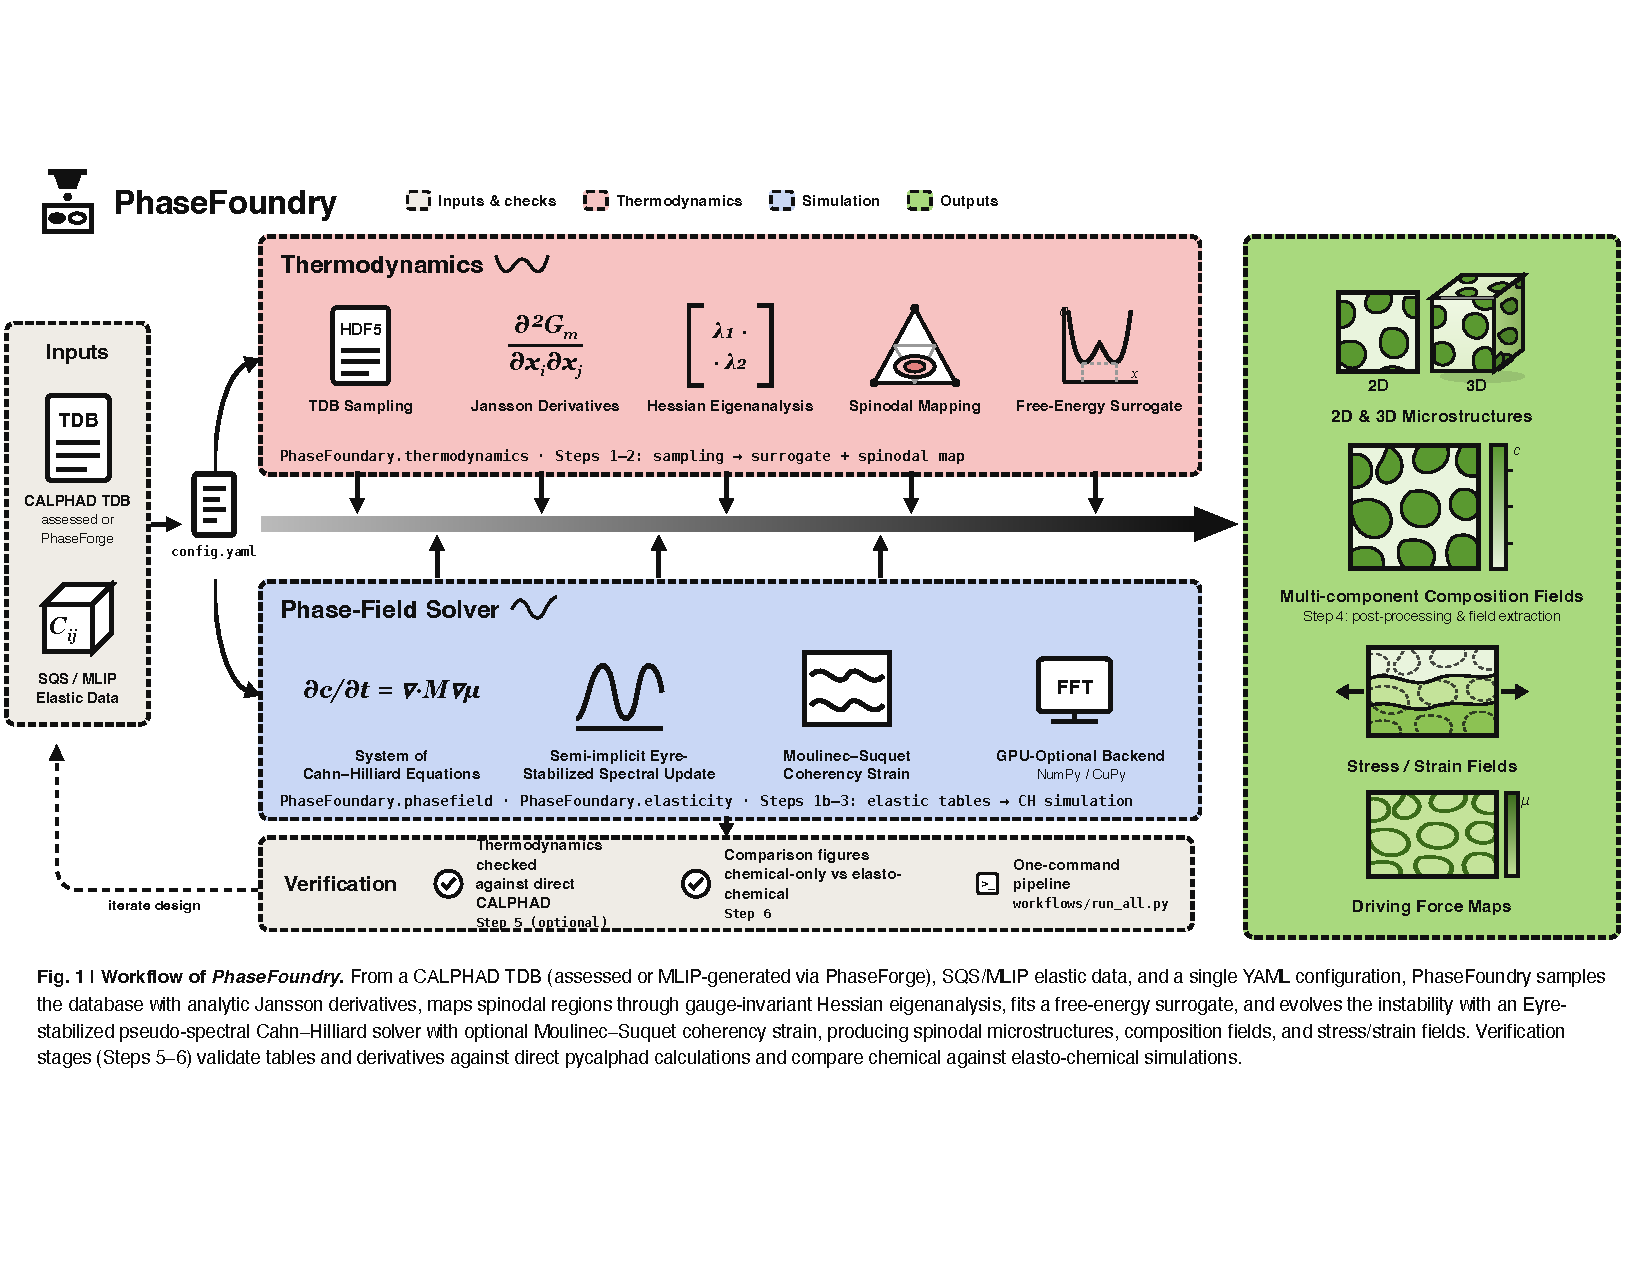
\includegraphics[angle=270, width=0.9\textwidth]{figs/PhaseFoundry.pdf}
  \caption{\textit{PhaseFoundry} workflow. Starting from a CALPHAD TDB (assessed or MLIP-generated via \textit{PhaseForge}), SQS/MLIP elastic data, and a YAML configuration file, the \emph{thermodynamics} subpackage (pink) samples Gibbs energy Hessians, fits a free-energy surrogate, and maps spinodal boundaries. The \emph{phasefield} subpackage (blue) evolves the instability via an Eyre-stabilized pseudo-spectral Cahn--Hilliard solver, optionally coupled to coherency strain through the \emph{elasticity} subpackage. Outputs (green) include composition, stress, and strain fields in 2D and 3D.}
  \label{fig:workflow}
\end{figure}

\begin{table}[H]
\centering
\caption{PhaseFoundry CLI entry points registered in \textit{pyproject.toml}. Each command maps to a specific subpackage and module within the \textit{phasefoundry} package.}
\label{tab:cli}
\scriptsize
\begin{tabular}{@{}ll>{\itshape}ll@{}}
\toprule
\textbf{Command} & \textbf{Subpackage} & \textbf{\upshape Module} & \textbf{Description} \\
\midrule
\textit{pf-generate}       & thermodynamics & calphad\_sampling           & Sample TDB over composition grid; write HDF5 tables \\
\textit{pf-surrogate}      & thermodynamics & free\_energy\_surrogate     & Fit free-energy surrogate; extract spinodal boundaries \\
\textit{pf-validate}       & thermodynamics & thermodynamic\_verification & Compare surrogate against direct \textit{pycalphad} queries \\
\textit{pf-elastic}        & elasticity     & elastic\_constants          & Build interpolant from SQS/MLIP elastic data \\
\textit{pf-tieline}        & elasticity     & eigenstrain\_reference      & Compute CALPHAD tie-line endpoints as Vegard eigenstrain reference states \\
\textit{pf-elastic-solve}  & elasticity     & elastic\_equilibrium        & Solve mechanical equilibrium via Lippmann--Schwinger iteration \\
\textit{pf-simulate}       & phasefield     & solver                      & Run pseudo-spectral Cahn--Hilliard simulation \\
\textit{pf-postprocess}    & phasefield     & visualize                   & Extract and plot composition, stress, and strain fields \\
\textit{pf-compare}        & phasefield     & solver                      & Compare chemical-only vs.\ elasto-chemical runs \\
\textit{pf-run-all}        & --             & pipeline                    & Execute the full pipeline in sequence \\
\bottomrule
\end{tabular}
\end{table}

\subsection{CALPHAD thermodynamic sampling}

The following command samples the CALPHAD thermodynamic database over a user-defined composition grid and stores the results as HDF5 tables:
\begin{lstlisting}[language=bash]
pf-generate --config configs/<alloy_config>.yaml
\end{lstlisting}
The configuration file specifies the TDB path, the alloy elements, the composition ranges, the number of grid points per axis, and the list of temperatures to evaluate. At each grid point, \textit{PhaseFoundry} calls \textit{pycalphad} to evaluate $G_m^\alpha$, the relative chemical potentials $\mu_i - \mu_n$, and their composition derivatives using the Jansson method. Results are written to an HDF5 file, one table per temperature. The number of grid points per axis controls the density of the thermodynamic sampling; values of 20 (ternary) and 10 (quaternary) are sufficient for accurate surrogate fitting in most cases. Three derivative modes are available via the \emph{derivative\_method} key: \emph{jansson} (default, analytic), \emph{finite\_diff}, and \emph{hybrid}.

\subsection{Elastic constant parameterization}

The following command tabulates SQS/MLIP elastic constants $C_{ij}$ and lattice parameters from \textit{PhaseForge} CSV outputs at the composition grid points:
\begin{lstlisting}[language=bash]
pf-elastic --config configs/<alloy_config>.yaml
\end{lstlisting}
The CSV file path is specified under the \emph{elastic.elastic\_csv} key. The script reads $C_{11}$, $C_{12}$, $C_{44}$, and the lattice parameter $a$ at each SQS composition, constructs an RBF interpolant over the quaternary composition space, and stores the interpolated values at all grid points. This table is consumed by Step~2 to build the elastic surrogate and by Step~3 to evaluate the Vegard eigenstrain at runtime. Step~1c (not shown) additionally invokes \textit{pycalphad} equilibrium calculations to determine the CALPHAD tie-line endpoint compositions at the simulation temperature, which are used to initialize the eigenstrain model.

\subsection{Free-energy surrogate and spinodal mapping}

The following command fits the free-energy surrogate and computes spinodal boundaries:
\begin{lstlisting}[language=bash]
pf-surrogate --config configs/<alloy_config>.yaml
\end{lstlisting}
The HDF5 thermodynamic tables from Step~1 are wrapped in a scattered-data interpolant (RBF with linear kernel by default), which is the only thermodynamic object queried at runtime. The Hessian $H_{ij}$ is evaluated at each grid point, transformed to a gauge-invariant Cartesian basis, and its eigenvalues are used to extract spinodal boundaries. The surrogate and spinodal data are saved to disk and loaded directly by Step~3.

\medskip
\noindent\textbf{Phase-map visualization (\texttt{pf-phase-map}).}
Two complementary visualization styles are available through the \texttt{thermo.phase\_map\_style} configuration key:

\begin{itemize}[leftmargin=1.5em,itemsep=2pt]
  \item \textbf{Ternary diagram} (\texttt{phase\_map\_style: ternary}, default for $n{=}3$).
        A standard Gibbs triangle rendered via \emph{python-ternary}, with
        single-phase, two-phase, and three-phase regions determined from the
        lower convex hull of $G_m$, and the spinodal boundary extracted from
        the negative-eigenvalue locus of $H_{ij}$.  For quaternary and
        higher-order systems, one projected ternary diagram is produced per
        unique pair of independent elements.

  \item \textbf{Alloy-Space UMAP} (\texttt{phase\_map\_style: umap}).
        Follows the AS-UMAP method of Vela \textit{et al.}\cite{vela2025visualizing}
        The full $n$-component composition simplex is grid-sampled at uniform
        increments, and the resulting point cloud is embedded in 2-D by UMAP
        (\emph{umap-learn}; \emph{scikit-learn} t-SNE used as fallback).
        When UMAP embeds the simplex correctly, ternary systems yield a
        deltoid (3-cusped hypocycloid) and quaternary systems yield an astroid
        (4-cusped hypocycloid), with each element vertex at a cusp and
        multi-component compositions in the interior.  CALPHAD data points are
        then overlaid and colored by phase region and spinodal label, providing
        a single, composition-topology-aware 2-D figure regardless of the
        number of components.

  \item \textbf{Both} (\texttt{phase\_map\_style: both}, default for $n{\ge}4$).
        Produces both the ternary projected diagrams and the AS-UMAP figure.
\end{itemize}

\subsection{Cahn--Hilliard phase-field evolution}

The following command runs the pseudo-spectral Cahn--Hilliard simulation:
\begin{lstlisting}[language=bash]
pf-simulate --config configs/<alloy_config>.yaml
\end{lstlisting}
The simulation is fully specified by the YAML configuration file. Key parameters include: the grid size \emph{N} (applied in each dimension for 2D or 3D), the domain side length \emph{Lx}, the gradient energy coefficients $\kappa_i$, the mobility matrix $M_{ij}$, the mean composition $c_0$, the time step \emph{dt} (or \emph{null} for automatic estimation), and the total number of steps \emph{n\_steps}. Setting \emph{use\_gpu: true} moves all FFT and array operations to a CUDA device via CuPy. For elasto-chemical runs, the \emph{elastic} block specifies the eigenstrain model (\emph{local\_vegard} or \emph{fixed\_vegard}), the elastic CSV path, the tie-line endpoints, and the solve frequency \emph{solve\_every}. Long runs write incremental NPZ checkpoints controlled by \emph{save\_every} and \emph{incremental\_npz}.

\subsection{Microstructure field extraction}

The following command extracts and visualizes composition, stress, and strain fields from simulation snapshots:
\begin{lstlisting}[language=bash]
pf-postprocess --config configs/<alloy_config>.yaml
\end{lstlisting}
The script reads the NPZ checkpoint file, computes derived fields (e.g., $x_V = 1 - \sum_i x_i$, von Mises stress), and writes publication-quality figures. Field snapshots at all saved time steps are available for animation or further analysis.

\subsection{Thermodynamic and microstructure verification}

Step~5 regenerates thermodynamic quantities directly from \textit{pycalphad} at randomly sampled compositions and compares them to the surrogate, quantifying interpolation error and the discrepancy between derivative modes:
\begin{lstlisting}[language=bash]
pf-validate --config configs/<alloy_config>.yaml
\end{lstlisting}
Step~6 runs matched chemical-only and elasto-chemical simulations from identical initial conditions, isolating the effect of coherency strain on the decomposition path and morphology:
\begin{lstlisting}[language=bash]
pf-compare --config configs/<alloy_config>.yaml
\end{lstlisting}
Both verification steps produce comparison figures that can be used to assess surrogate accuracy and the magnitude of elastic effects before committing to a long production run.



%% ── 4. Configuration file and workflow setup ─────────────────────
\section{Configuration file and workflow setup}
\label{sec:config}

All \textit{PhaseFoundry} pipeline steps are governed by a single YAML configuration file. The identical file is consumed by every \emph{pf-*} command in sequence, so no additional input is required at any stage; archiving it alongside simulation outputs is sufficient for full reproducibility. The file is organized into four top-level blocks. The \emph{system} block identifies the alloy, TDB path, constituent elements, target phase, and reference element. The \emph{thermo} block defines the composition grid, sampling density, and temperatures for CALPHAD evaluation. The \emph{simulation} block governs spatial discretization, time-stepping, the gradient energy coefficient $\kappa$, mobility matrix $M$, mean composition $c_0$, thermodynamic derivative mode, and the optional \emph{elastic} sub-block for elasto-chemical coupling. The \emph{output} block sets data and results directories and the run identifier. Fig.~\ref{lst:config} shows the full configuration reference with all supported keys; a minimal binary starting point is provided as \texttt{config/template.yaml} in the repository.

The \emph{derivative\_method} key controls how the Gibbs energy Hessian is evaluated. The \emph{jansson} mode computes exact analytic derivatives via the Jansson method in \textit{pycalphad} and is the recommended default for speed and accuracy. The \emph{fd} mode uses finite differences and serves as a fallback for TDB models not yet supported analytically or for cross-validation. The \emph{hybrid} mode applies \emph{jansson} where it converges and falls back to \emph{fd} otherwise.

When elasto-chemical coupling is active, the \emph{elastic} sub-block must be provided. The \emph{stiffness\_model} key selects between a composition-independent isotropic approximation (\emph{isotropic}) and a composition-dependent cubic stiffness tensor interpolated from SQS or MLIP data (\emph{cubic\_csv}). The \emph{c\_mat} and \emph{c\_ppt} keys supply the tie-line endpoint compositions that define the Vegard eigenstrain reference states; these are produced by a prior \emph{pf-tieline} run and stored in \texttt{elastic\_params.yaml}. Setting \emph{warm\_start} to \texttt{true} reuses the displacement field from the previous elastic solve as an initial guess, substantially reducing iteration counts in slowly evolving microstructures.

\begin{figure}[H]
\centering
\begin{lstlisting}[language=yaml]
system:
  name:              <alloy_name>
  db_path:           data/tdb/<database>.tdb
  elements:          [EL1, EL2, EL3]  # last = reference
  phase:             <phase_name>
  reference_element: EL3

thermo:
  composition_ranges:
    EL1: [<x_min>, <x_max>]
    EL2: [<x_min>, <x_max>]
  n_points:        <n>   # 20 (ternary), 10 (quaternary)
  temperatures_C:  [<T1>, <T2>]

simulation:
  temperature_C:     <T>
  dimensions:        2        # 2 | 3
  N:                 <N>      # grid points per axis
  Lx:                <Lx>     # domain size [m]
  kappa:             [<k1>, <k2>]  # J m^2/mol per field
  M:                 [[<M11>, <M12>],
                      [<M21>, <M22>]]
  c0:                [<c1>, <c2>]  # mean mole fractions
  derivative_method: jansson  # fd|jansson|hybrid
  dt:                null     # null = auto
  adaptive_dt:       false
  noise:             <sigma>
  seed:              <int>
  n_steps:           <n_steps>
  save_every:        <save_every>
  incremental_npz:   false
  use_gpu:           false
  elastic:
    enabled:           true
    stiffness_model:   cubic_csv  # isotropic|cubic_csv
    eigenstrain_model: fixed_vegard  # fixed|local
    elastic_csv:       data/<alloy>/elastic_params.yaml
    c_mat:             [<x1_mat>, <x2_mat>]
    c_ppt:             [<x1_ppt>, <x2_ppt>]
    solve_every:       10
    warm_start:        true
    tol:               1.0e-6
    max_iter:          200

output:
  data_dir:    data/<alloy_name>
  results_dir: results/<alloy_name>
  run_name:    auto
\end{lstlisting}
\caption{\textit{PhaseFoundry} YAML configuration reference. Angle-bracket tokens are user-supplied values; optional keys carry the defaults shown. A minimal binary template is provided as \texttt{config/template.yaml} in the repository.}
\label{lst:config}
\end{figure}

Table~\ref{tab:config} summarises how the configuration evolves from binary to ternary and quaternary systems. Adding a component extends the list-valued keys ($\kappa$, $c_0$) and promotes the scalar mobility \emph{M} to a full $n{\times}n$ matrix, where off-diagonal entries encode solute--solute cross-diffusion. For refractory HEAs, diffusivities can span orders of magnitude across elements, and the diagonal mobility matrix accommodates this directly.

\begin{table*}[!h]
\centering
\caption{Configuration key values for three representative alloy systems of increasing complexity: binary Hf--Nb, ternary Nb--Hf--V, and quaternary Hf--Nb--Ti--V with elasto-chemical coupling. Keys marked ``--'' are absent or not applicable for that system. All three systems share the same \emph{phase}, \emph{output}, and solver control keys.}
\label{tab:config}
\scriptsize
\begin{tabular}{@{}ll p{2.0cm} p{2.2cm} p{2.8cm} p{3.8cm}@{}}
\toprule
\textbf{Block} & \textbf{Key} & \textbf{Binary (Hf--Nb)} & \textbf{Ternary (Nb--Hf--V)} & \textbf{Quaternary + elastic (Hf--Nb--Ti--V)} & \textbf{Notes} \\
\midrule
system  & elements            & \texttt{[HF, NB]}        & \texttt{[NB, HF, V]}          & \texttt{[NB, HF, TI, V]}         & last = reference \\
system  & reference\_element  & \texttt{NB}              & \texttt{V}                    & \texttt{V}                       & dependent variable \\
\midrule
thermo  & composition\_ranges & 1 entry (HF)             & 2 entries (NB, HF)            & 3 entries (NB, HF, TI)           & one per indep.\ field \\
thermo  & n\_points           & 200                      & 20                            & 10                               & per axis \\
\midrule
simulation & $\kappa$          & scalar                   & 2-list                        & 3-list                           & J m$^2$/mol per field \\
simulation & M                & scalar                   & $2{\times}2$ matrix           & $3{\times}3$ matrix              & m$^5$/(J s); diag.\ = self-diff. \\
simulation & $c_0$            & scalar                   & 2-list                        & 3-list                           & mole fractions; $x_{\rm ref} = 1 - \sum$ \\
simulation & derivative\_method & \texttt{fd}            & \texttt{fd}                   & \texttt{jansson}                 & fd / jansson / hybrid \\
simulation & dt               & \texttt{null}            & \texttt{null}                 & \texttt{5e-1}                    & null = auto from $\max|H_{ii}|$ \\
simulation & n\_steps         & 100\,000                 & 30\,000                       & 3\,000\,000                      & \\
simulation & incremental\_npz & \texttt{false}           & \texttt{false}                & \texttt{true}                    & streaming checkpoints \\
\midrule
elastic & enabled             & --                       & --                            & \texttt{true}                    & activates Moulinec--Suquet solver \\
elastic & stiffness\_model    & --                       & --                            & \texttt{cubic\_csv}              & RBF from SQS/MLIP data \\
elastic & c\_mat / c\_ppt     & --                       & --                            & tie-line endpoints               & Vegard eigenstrain ref. states \\
elastic & solve\_every        & --                       & --                            & 10                               & CH steps between elastic solves \\
elastic & warm\_start         & --                       & --                            & \texttt{true}                    & re-uses previous displacement \\
\midrule
output  & run\_name           & \texttt{auto}            & \texttt{auto}                 & \texttt{auto}                    & pattern: \texttt{pf\_c\{comp\}\_\{tdb\}} \\
\bottomrule
\end{tabular}
\end{table*}

%% ── 5. Illustrative applications ─────────────────────────────────
\section{Examples}
\label{sec:apps}

In this section, the workflow steps described in Section~\ref{sec:usage} are illustrated for three alloy systems of increasing complexity: a binary Nb--V reference case, a ternary Nb--Hf--V system, and a quaternary Hf--Nb--Ti--V HEA. Together, these examples demonstrate that the same package, solver, and post-processing scripts handle every system; only the YAML configuration file changes.

\textbf{Binary Nb--V.} The Nb--V BCC\_A2 system serves as the reference case. Chemical-only simulations at \SI{500}{\degreeCelsius} across mean compositions $x_{\mathrm{Nb}} = 0.3$--$0.8$ show the expected progression from isolated to bicontinuous morphologies in 2D ($128^2$) and 3D ($128^3$) domains. All three derivative modes (fd, jansson, hybrid) agree closely across the full composition range.

\textbf{Ternary Nb--Hf--V.} With two independent composition fields and anisotropic mobilities, the ternary case demonstrates multicomponent capability. Fig.~\ref{fig:ternary} shows the spinodal instability region at \SI{500}{\degreeCelsius} identified by \emph{pf-surrogate} through gauge-invariant Hessian eigenanalysis, alongside the Nb composition field from a $128^2$ simulation at the marked composition ($x_{\mathrm{Nb}} = 0.50$, $x_{\mathrm{Hf}} = 0.25$). The bicontinuous spinodal morphology is fully resolved; only the YAML configuration changes relative to the binary case.

\clearpage
\begin{figure}[H]
  \centering
  % Row 1: phase maps (binary, ternary, quaternary 
  \begin{overpic}[width=0.30\linewidth]{figs/phase_diagram.png}
    \put(2,75){\colorbox{white!60}{\textbf{(a)}}}
  \end{overpic}
  %
  \begin{overpic}[width=0.30\linewidth]{figs/nbhfv_phase_map.pdf}
    \put(2,75){\colorbox{white!60}{\textbf{(b)}}}
  \end{overpic}
  %
  \begin{overpic}[width=0.30\linewidth]{figs/nbhftiv_phase_map.pdf}
    \put(2,75){\colorbox{white!60}{\textbf{(c)}}}
  \end{overpic}
  % Row 2: teranry microstructure Ichem-only and elastochemical
  \begin{overpic}[width=0.40\linewidth]{figs/nbhfv_microstructure.pdf}
    \put(2,96){\colorbox{white!60}{\textbf{(b)}}}
  \end{overpic}
  \par\smallskip
  % Row 3: derivative comparison (full width)
  \begin{overpic}[width=0.98\linewidth]{figs/nbhfv_derivative_comparison.pdf}
  \end{overpic}
  \caption{Ternary Nb--Hf--V BCC\_A2 pipeline outputs at \SI{500}{\degreeCelsius} ($x_{\rm Nb} = 0.45$, $x_{\rm Hf} = 0.20$). (a)~Spinodal instability map from \emph{pf-phase-map}: orange shading marks two-phase regions; dashed contour is the spinodal boundary ($\lambda_{\min}(H) < 0$); star marks the simulated composition. (b)~Composition microstructure from \emph{pf-postprocess}: main panel shows $x_V$; insets show $x_{\rm Nb}$ and $x_{\rm Hf}$ for the highlighted crop region. (c)~Derivative method comparison from \emph{pf-validate}: molar Gibbs energy $G_m$, relative chemical potential $\mu_{\rm Nb}-\mu_{\rm V}$, and Hessian $\partial^2 G/\partial x_{\rm Nb}^2$ computed by finite-difference, Jansson, and hybrid modes, overlaid on CALPHAD data along the $x_{\rm Hf}=0.20$ slice; shaded band marks the spinodal region ($H<0$).}
  \label{fig:ternary}
\end{figure}

\textbf{Quaternary Hf--Nb--Ti--V.} The equiatomic elasto-chemical configuration runs $3 \times 10^6$ time steps with three coupled composition fields, MLIP-derived composition-dependent stiffness, and tie-line endpoints from \emph{pf-tieline} informed by the XRD phase compositions of An~\textit{et al.}\cite{an2021spinodal} Scientific analysis of the results appears in the companion paper.\cite{kunselman2025spinodal}


%% ── 5. Relation to existing software ─────────────────────────────
%% ── 6. Conclusions ───────────────────────────────────────────────
\section{Conclusions}

We presented \textit{PhaseFoundry}, an open-source Python framework that automates the path from a CALPHAD thermodynamic database to quantitative spinodal microstructure predictions in multicomponent alloys. The utility of the framework is twofold. First, it provides a rigorous and reproducible method for coupling CALPHAD free energies to phase-field simulations: analytic Jansson derivatives eliminate finite-difference approximation errors in the Gibbs energy Hessian, and gauge-invariant eigenanalysis maps spinodal instability regions without artifact from the choice of dependent component. Second, the framework extends naturally to elasto-chemical systems: MLIP-derived, composition-dependent elastic constants are interpolated over the full composition space, and a Moulinec--Suquet spectral solver computes coherency stresses at runtime with the same YAML configuration that governs the thermodynamic pipeline.

The presented tools are among the few open-source efforts to couple CALPHAD databases directly to pseudo-spectral phase-field solvers for multicomponent alloys, and the only one to integrate MLIP-generated elastic constants and Vegard eigenstrain models in a unified workflow. Some aspects of the implementation could be improved in the future: mobility matrices are currently user-supplied constants, and coupling to CALPHAD kinetic databases (DICTRA-style) is a natural next step. Together with \textit{PhaseForge}, \textit{PhaseFoundry} completes an open-source chain from machine-learned interatomic potentials to microstructure for HEA design.

%% ── Data and code availability ───────────────────────────────────
\section*{Data and code availability}

\textit{PhaseFoundry} is available under the MIT license at \url{https://github.com/vahid2364/PhaseFoundry}, including all YAML configurations, workflow scripts, SQS/MLIP elastic constant tables, and post-processing scripts. Thermodynamic databases were generated with \textit{PhaseForge}\cite{sariturk2025phaseforge} (DOI:~10.5281/zenodo.15730911).

%% ── Author contributions ─────────────────────────────────────────
\section*{Author contributions}

V.A.: conceptualization, software, methodology, validation, visualization, writing (original draft). R.A.: funding acquisition, supervision, writing (review and editing).

%% ── Conflicts of interest ────────────────────────────────────────
\section*{Conflicts of interest}

There are no conflicts of interest to declare.

%% ── Acknowledgements ─────────────────────────────────────────────
\section*{Acknowledgements}

The authors acknowledge support from the Army Research Office (Grant No.\ W911NF-22-2-0117) and the National Science Foundation.

%% ── References ───────────────────────────────────────────────────
\bibliographystyle{unsrtnat}
\bibliography{paper}

\end{document}
